\section{Analyzing longitudinally collected isolates from patients of the University hospital Basel}
\subsection{Sample collection and selecting patients of interest}
Adrian Eglis group collected 65 isolates from 34 patients over a time span of approximately four and a half years.
Sample collection from one patient happened within several months. In order to find out that a certain patient was infected with the same strain over the sample period a phylogenic tree was build with panX which visualizes how closely related the pan genome of different isolates is. This was done by assembling every isolate with its short-read Illumina sequences provided by Adrian Egli using spades (v3.12.0) \cite{spades}.
Every resulting assembly was annotated using prokka (v.1.12) \cite{prokka}. The genbank file returned from prokka was used to run panX \cite{panx}. 

\subsection{Sequencing and assembling of the reference genome}
\label{section:reference_genome}
\subsubsection{Nanopore sequencing}
Every sample of interest (\ref{table:samples_overview}) was sequenced with a MinION from Oxford Nanopore. Each library was prepared with a ligation sequencing kit (LSK-108) followed with the native barcoding expansion kit allowing barcoding every sample and loading all of them on a single flow cell (FLO-MIN106D). A detailed description of the protocol is available in Nicholas Noll publication \cite{nanopore}.

\subsubsection{Illumina sequencing}
Illumina sequencing was done by our collaborator Adiran Egli from the University hospital of Basel. His team extracted the DNA from cultured isolates using the EZ1 DNA tissue kit on an EZ1 Advanced XL robotic system (Qiagen). The library for the sequencing was prepared using the Nextera XT library preparatino kit (Illumina). The resulting library was sequenced using a MiSeq Illumina platform \cite{nanopore}.

\subsubsection{Assembling of the reference gemoe}
Before assembling trimming was performed for all the Illumina reads using Trim Galore \cite{trim_galore}.
Both sequencing data from Illumina and Nanopore were combined into a hybrid assemly using Unicycler \cite{unicycler}. This was done for every isolate with the lowest MICs for every patient and defined as reference genome.

\subsection{Identifying SNPs}
Based on the reference genome built according to the section \ref{section:reference_genome} pile ups were created with every sample for each patient. This means, that the Illumina reads for every isolate of each patient were mapped to the reference genome which was stored as a bam-file. As a mapper 
BWA MEM \cite{bwa_mem} was used. 
The pile ups were produced with a custom script written by Richard Neher.
The script iterated over every position in the reference genome. Then it checked which base was present in every read which was mapped to this position, using the CIGAR-code of the read. This resulted in a count matrix for every position in the reference genome allowing to calculate base frequency and the coverage for every position. The python pileup.py script used to produce the pile ups is available on \href{https://github.com/nahanoo/ESBL\_project/pileup.py}{GitHub}.

Pile ups in form of count matrices were calculated for every sample. Since they were produced using the same reference sequence per patient, all the pile ups for each contig from every sample could be stored in one matrix, giving a list of matrices per patient. This was very handy, because this data structure allowed to easily compare positions over different samples.

Using the pile ups every position for every patient was checked for variance with another script called \href{https://github.com/nahanoo/ESBL\_project/pileup.py}{analysis\_modular.py}. Since many positions showed variance caused by sequencing and mapping errors filtering was applied by setting a threshold for coverage and base frequency. As such thresholds 30 was chosen for the minimum coverage and 0.8 for the minimum base frequency. 

\subsubsection{Annotating the genomes}
In order to possibly find out what in in the genome is affected by the SNPs, the genes were identified using prokka \cite{prokka}. Additionally promoters were classified using the promoter prediction tool PePPER \cite{pepper} and the promoter data base hosed on EcoCyc \cite{ecocyc}. With this annotation it was possible to identify some genes and promoters altered by SNPs.

\section{Assembling and handling procedure of the morbidostat}
Initially the first morbidostat was build by Toprak et al. \cite{morb_toprak}. The following system is an adapted version of Topraks built differing mainly in it's pump system, controlling unit and software. Hardware which was not commercially available was built by the in-house mechanic and electronic workshop.

\subsection{Hardware and setup}

\begin{figure}[H]
	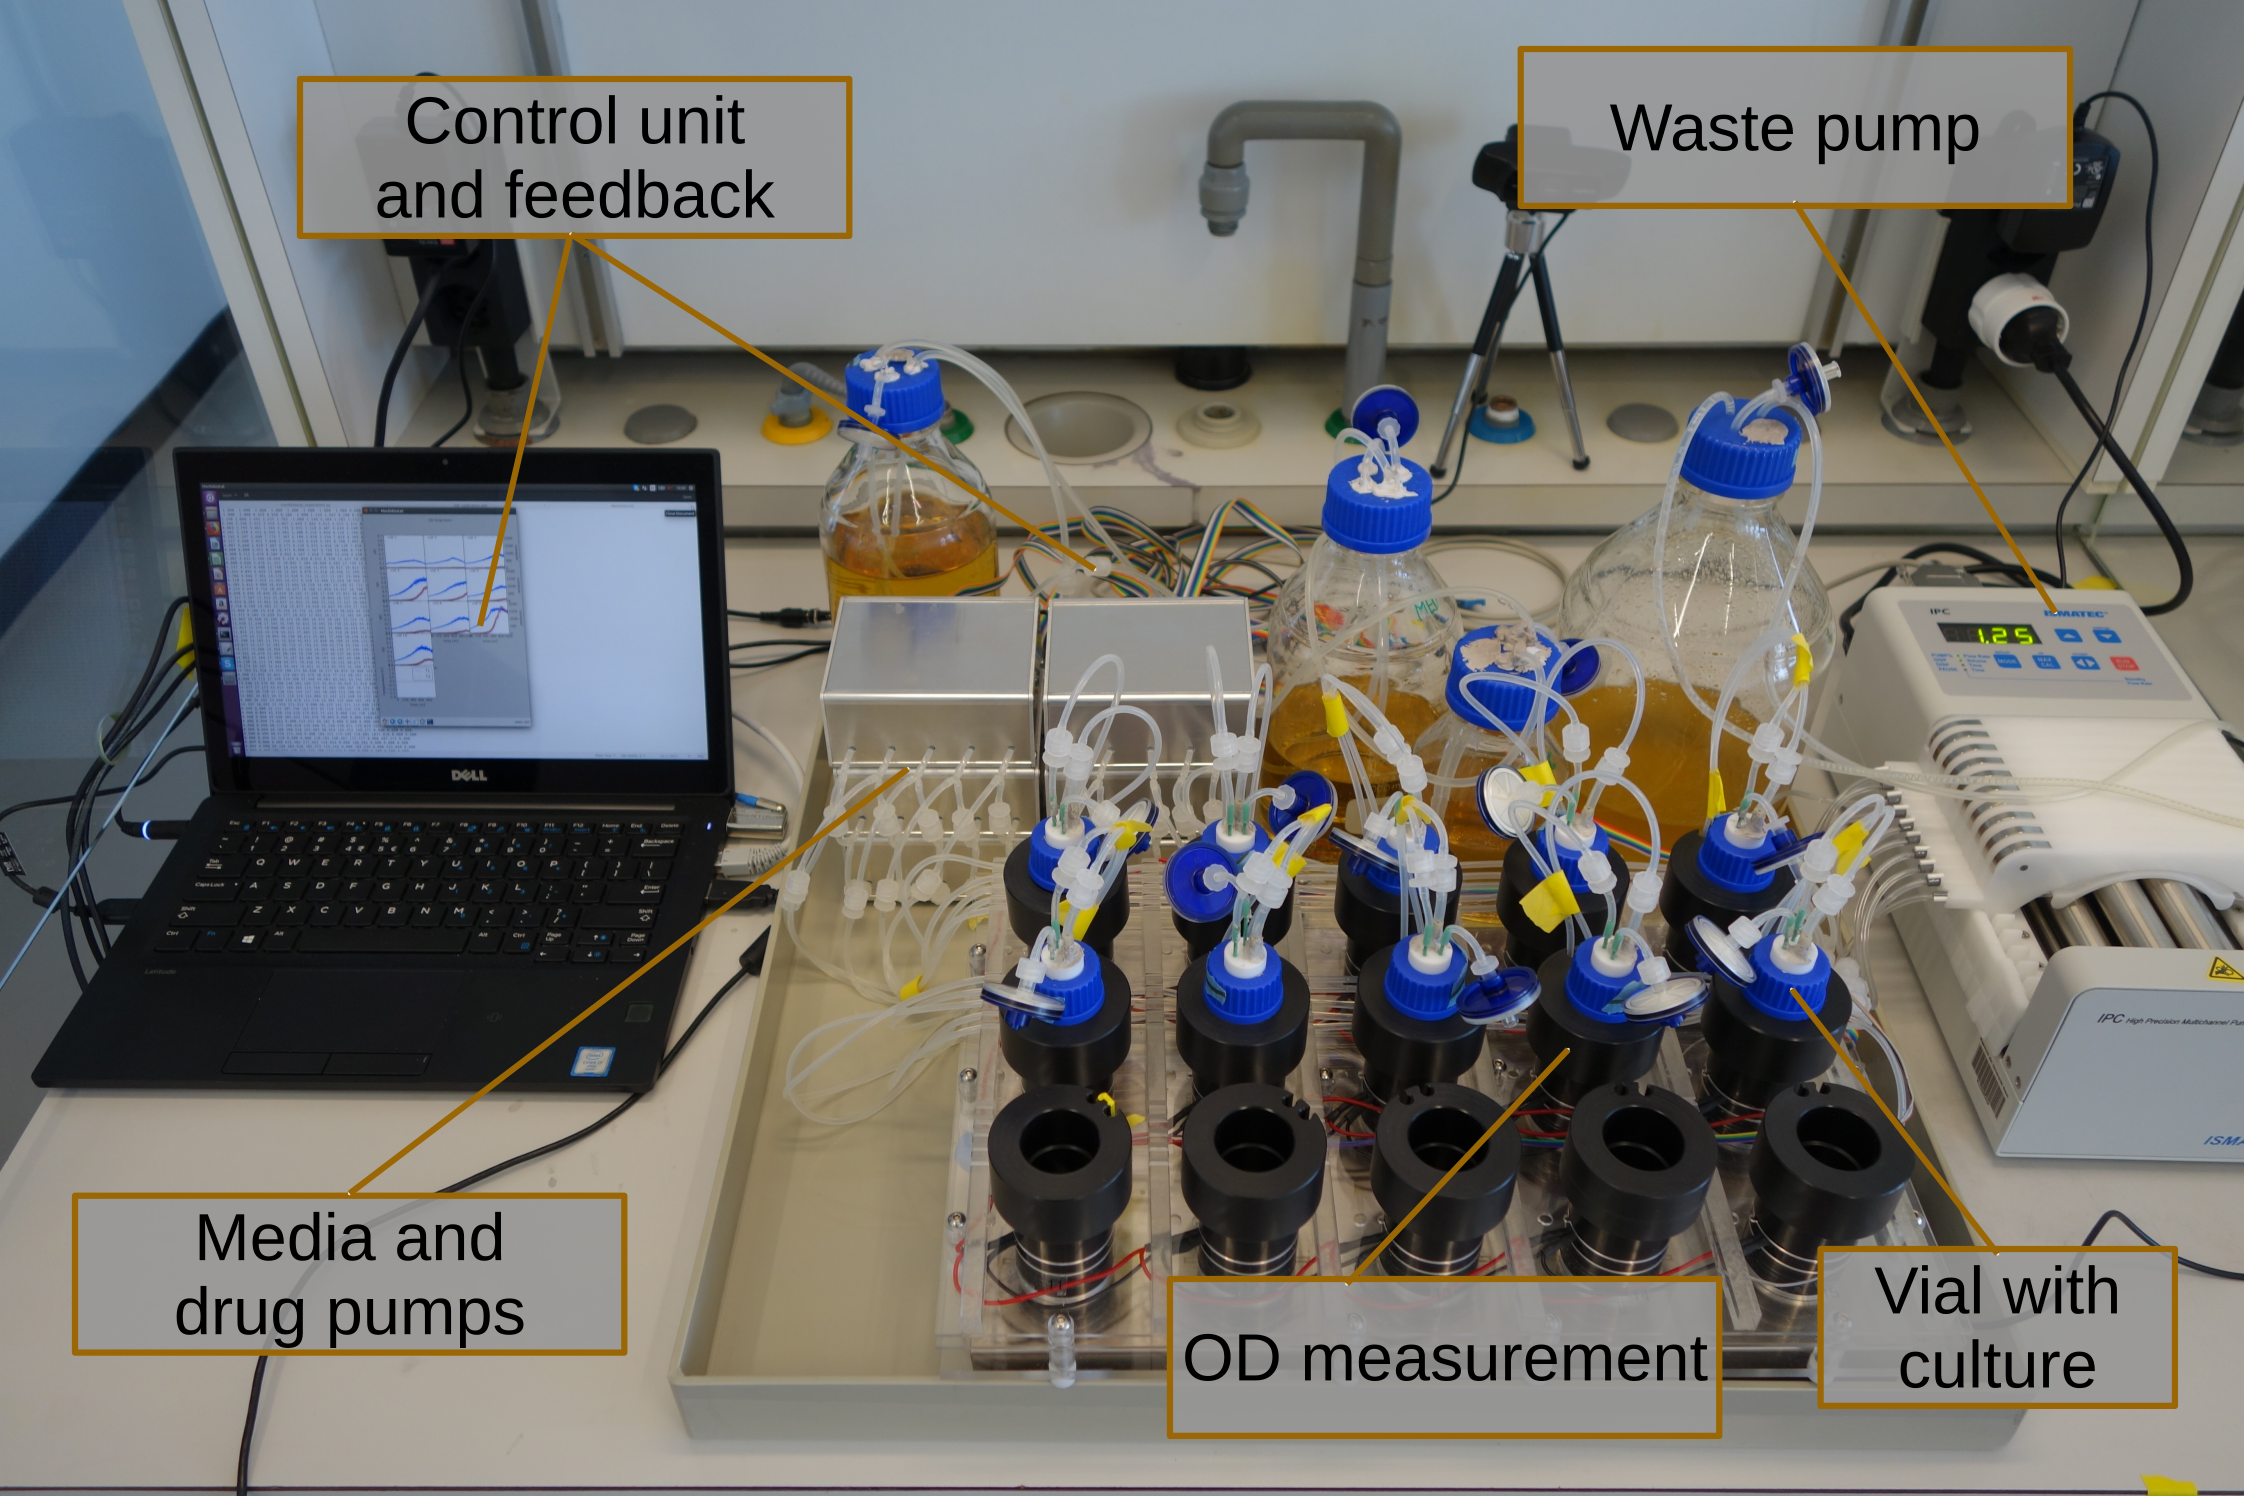
\includegraphics[scale=0.7]{setup_annotated_inksacpe.png}
	\caption{Overview of the morbidostat setup. Behind the drug and media pumps the arduino is located.}
	\label{figure:morbidostat_setup}
\end{figure}  
In Figure \ref{figure:morbidostat_setup} the morbidostat setup is shown. Only 10 cultures were used but potentially 15 cultures can be monitored and inhibited with this setup. On the magnetic stirrer which caused constant mixing the electronics for measuring the OD was placed integrated in a vial holder. In this holder the vials sit and were connected to a media bottle, two drug bottles with different concentrations, one waste pump and an air filter. The connection was made using silicon tubing and plastic luers. For controlling the hardware an arduino was used, who processed information and executed commands fed from a python program which ran on a laptop. 
In Figure \ref{figure:morbidostat_setup} the morbidostat was built up in the open, for later experiments the morbidostat was placed in an hypoxi-station within a biosafety level 2 lab. This was necessary in order for temperature regulation but also for safety reasons.  

\subsubsection{OD measurements}
For measuring the OD a combination of a light emitting diode and a phototransistor was chosen. The principle is, that at lower ODs more light could get through the culture which caused a bigger opening in the semiconductor from the phototransitor. This led to more flowing current in the base region, which could be detected with the Arduino. Since a current was detected this implemented, that a calibration was necessary in order that the translation to an OD could be done.\\
As a light emitting diode OPB608A was chosen from TT electronics with a peak wavelength of 890 nm. For detection a PT 333-3C phototransistor was used. The 15 OD-measuring installations have been split up into three parallel-connected chains representing one row of 5 vials. Each chain was connected to a 5 V power supply and grounded as shown in Figure \ref{figure:OD_cirguit}. To limit the current a resistor of ? \textOmega \space was added for every chain. The current was getting measured by an analog pin, which was connected to a shield mounted on the arduino. In order that sensitivity could be changed a potentiometer was added in serial before the current measurement. It turned out that the system was not as sensitive as thought in advance, so all the potentiometers were opened as much as possible.   

\begin{figure}
	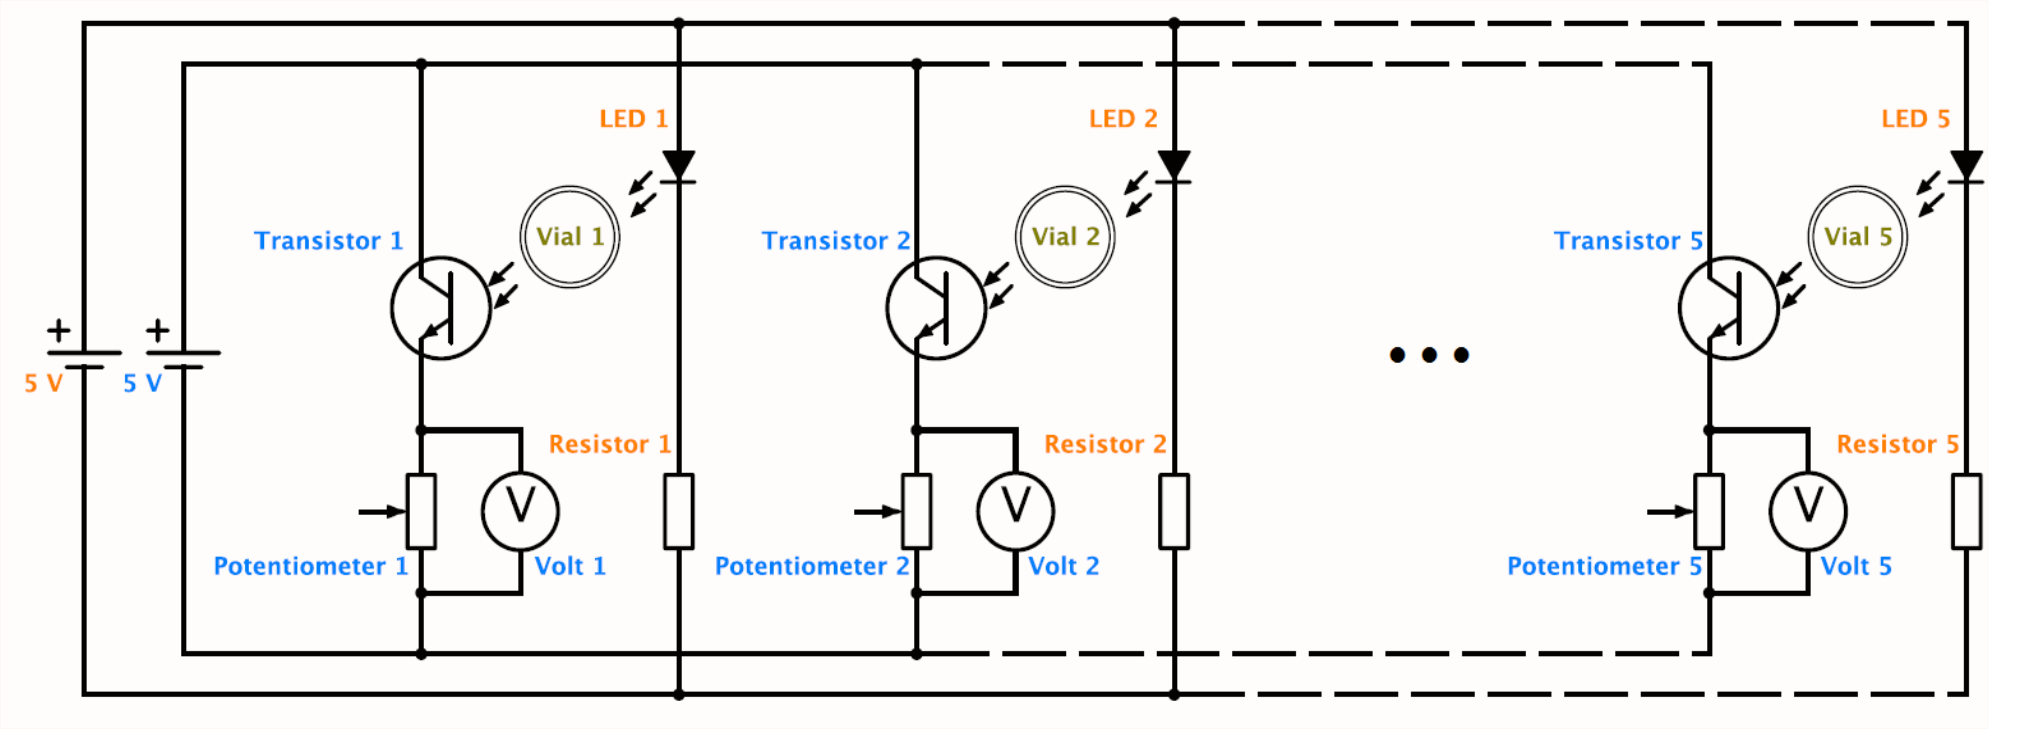
\includegraphics[scale=0.15]{OD_setup.png}
	\caption{Left figure: Circuit diagram of parallel-connected LED (orange) and phototransistors (blue). This circuit is done independently three times for five vials each. The detector and the LED are orientated in a 135 \degree  angle since this is the best angle for light detection. Right figure: vial setup}
	\label{figure:OD_cirguit}
\end{figure}

\subsubsection{Vials and tubing}
Every vial was connected to three injecting pumps and one pump which sucked off the waste, meaning every volume which was above the desired culture volume as shown in Figure \ref{figure:tubing_setup}. The three injecting pumps were able to inject media or two different drug concentrations. Since it was a lot easier to make one inlet in the vial instead of three, the tubes which are injecting fluid were connected before the vial, leading to only one inlet. Because fluid getting added an air filter had to be mounted, necessary for equalizing air pressure.   

\subsubsection{Pumps} 
\begin{figure}
	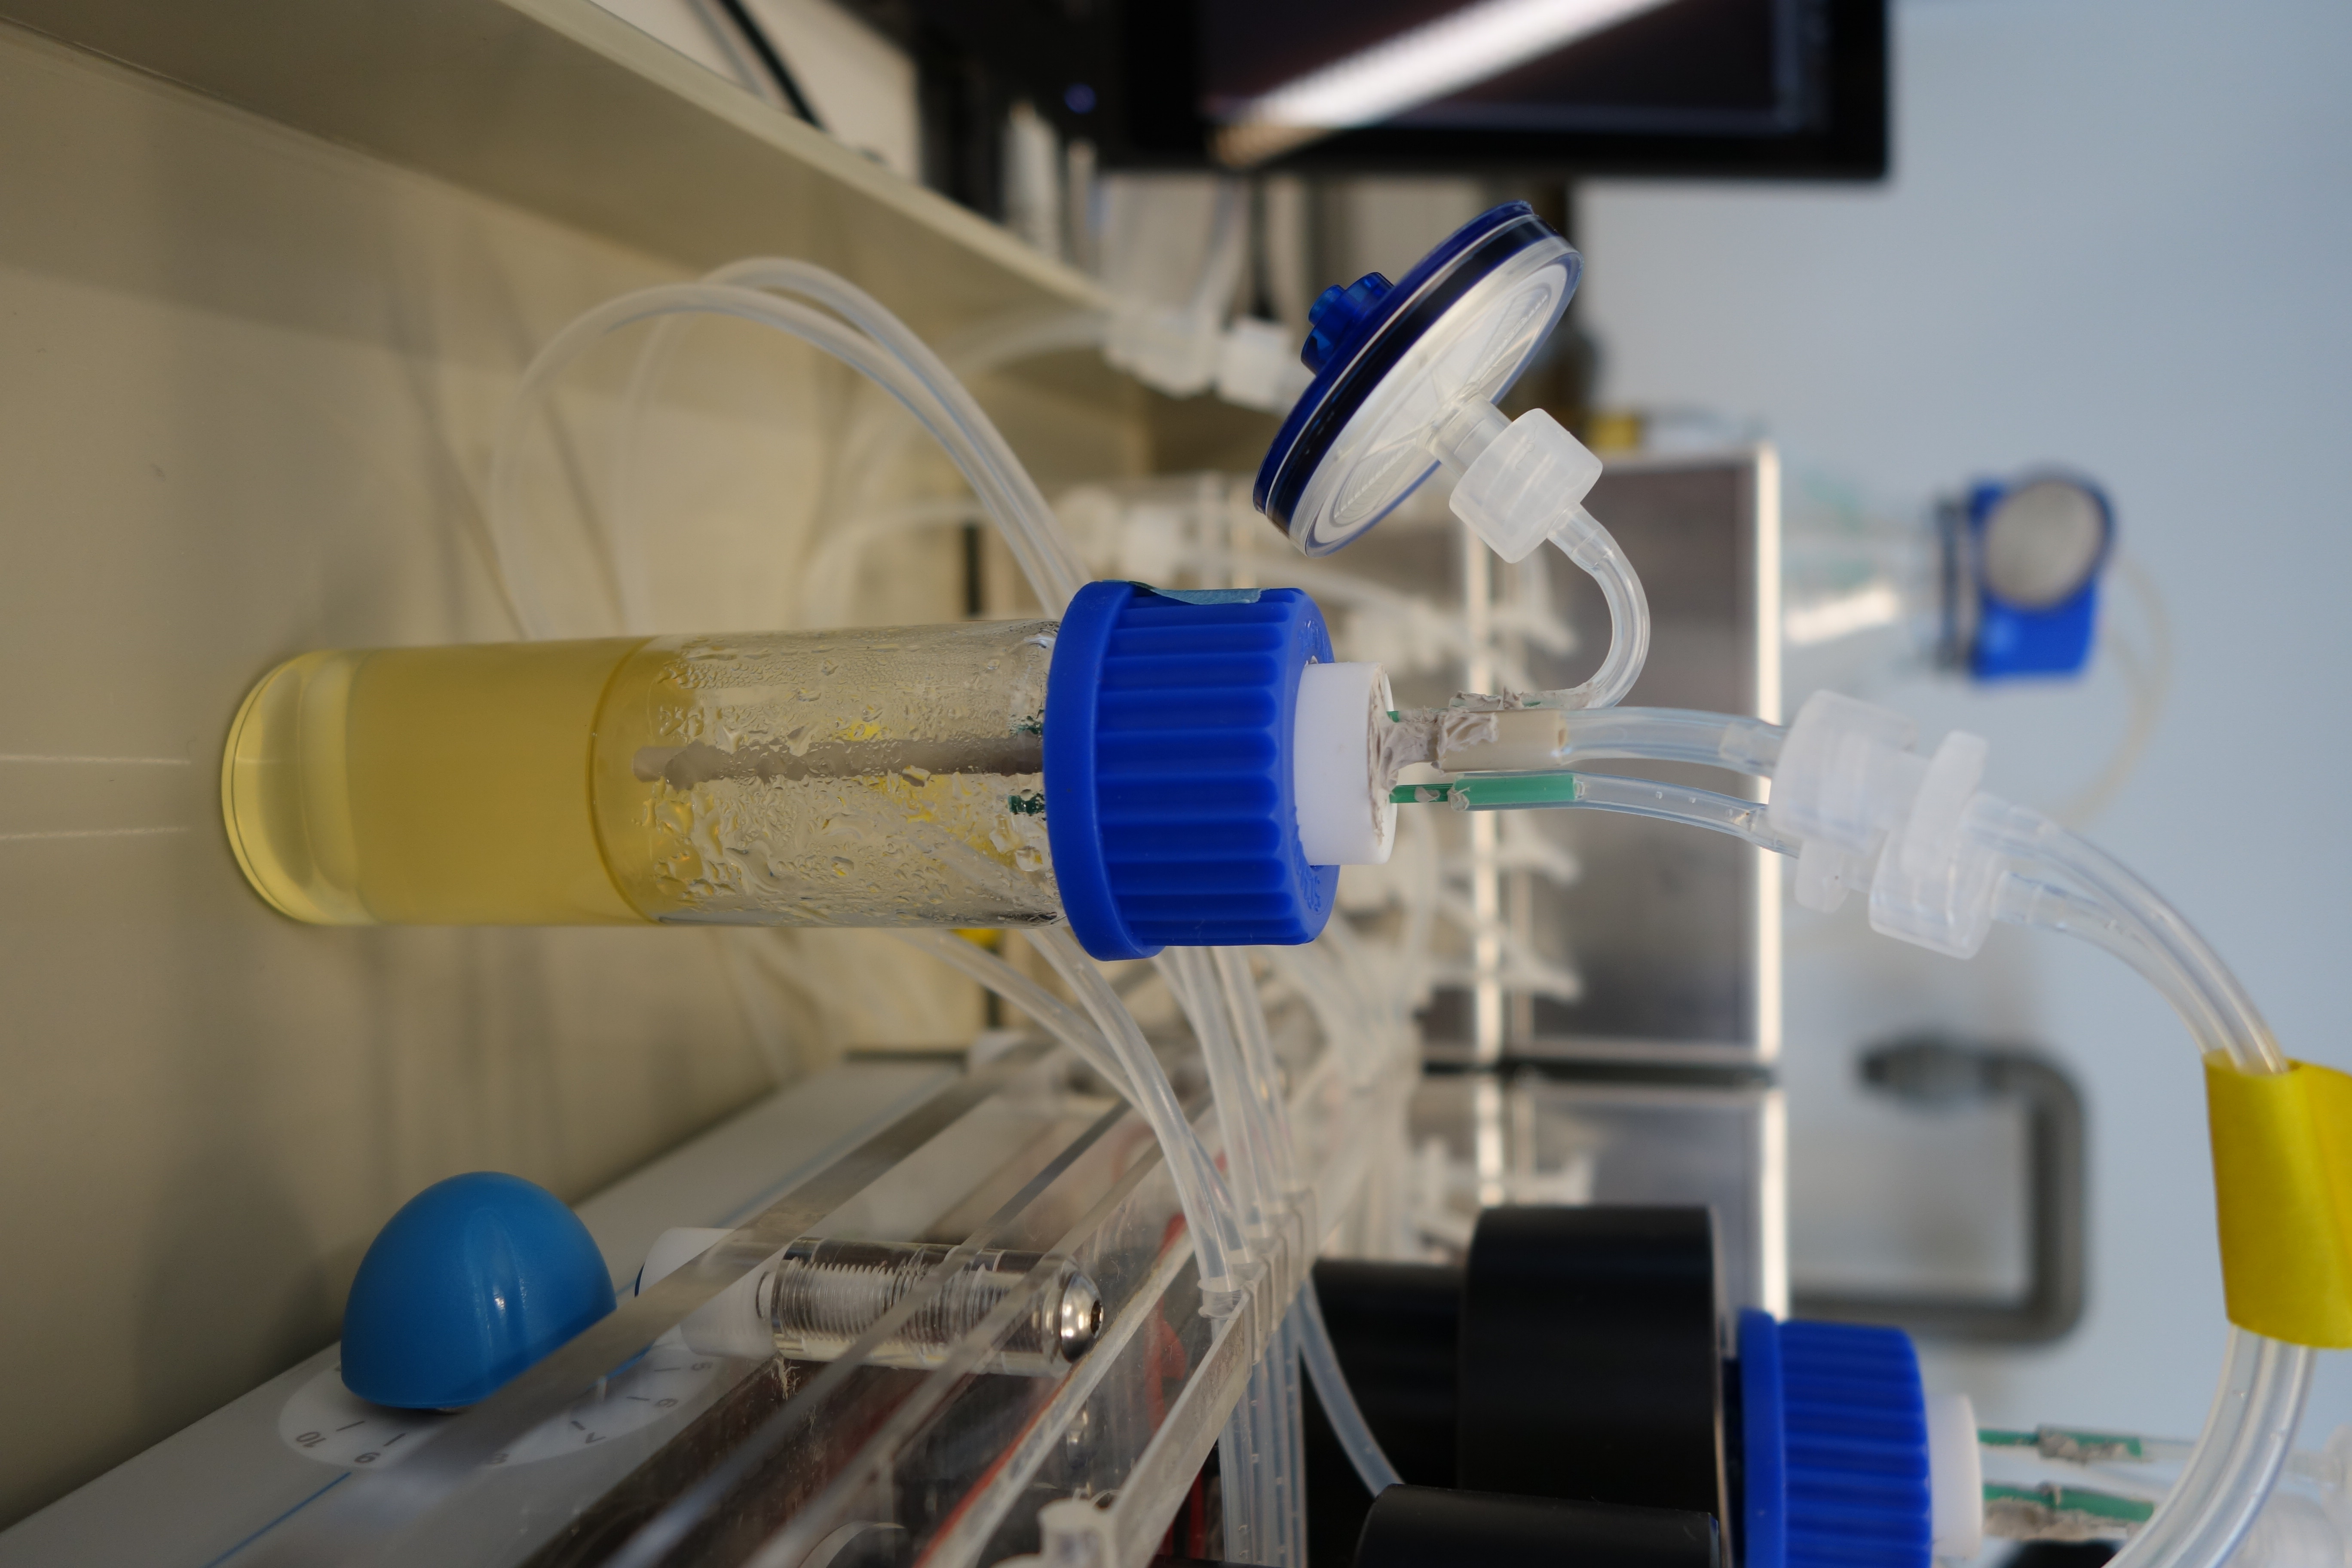
\includegraphics[angle=90,scale=0.15]{vial.JPG}
	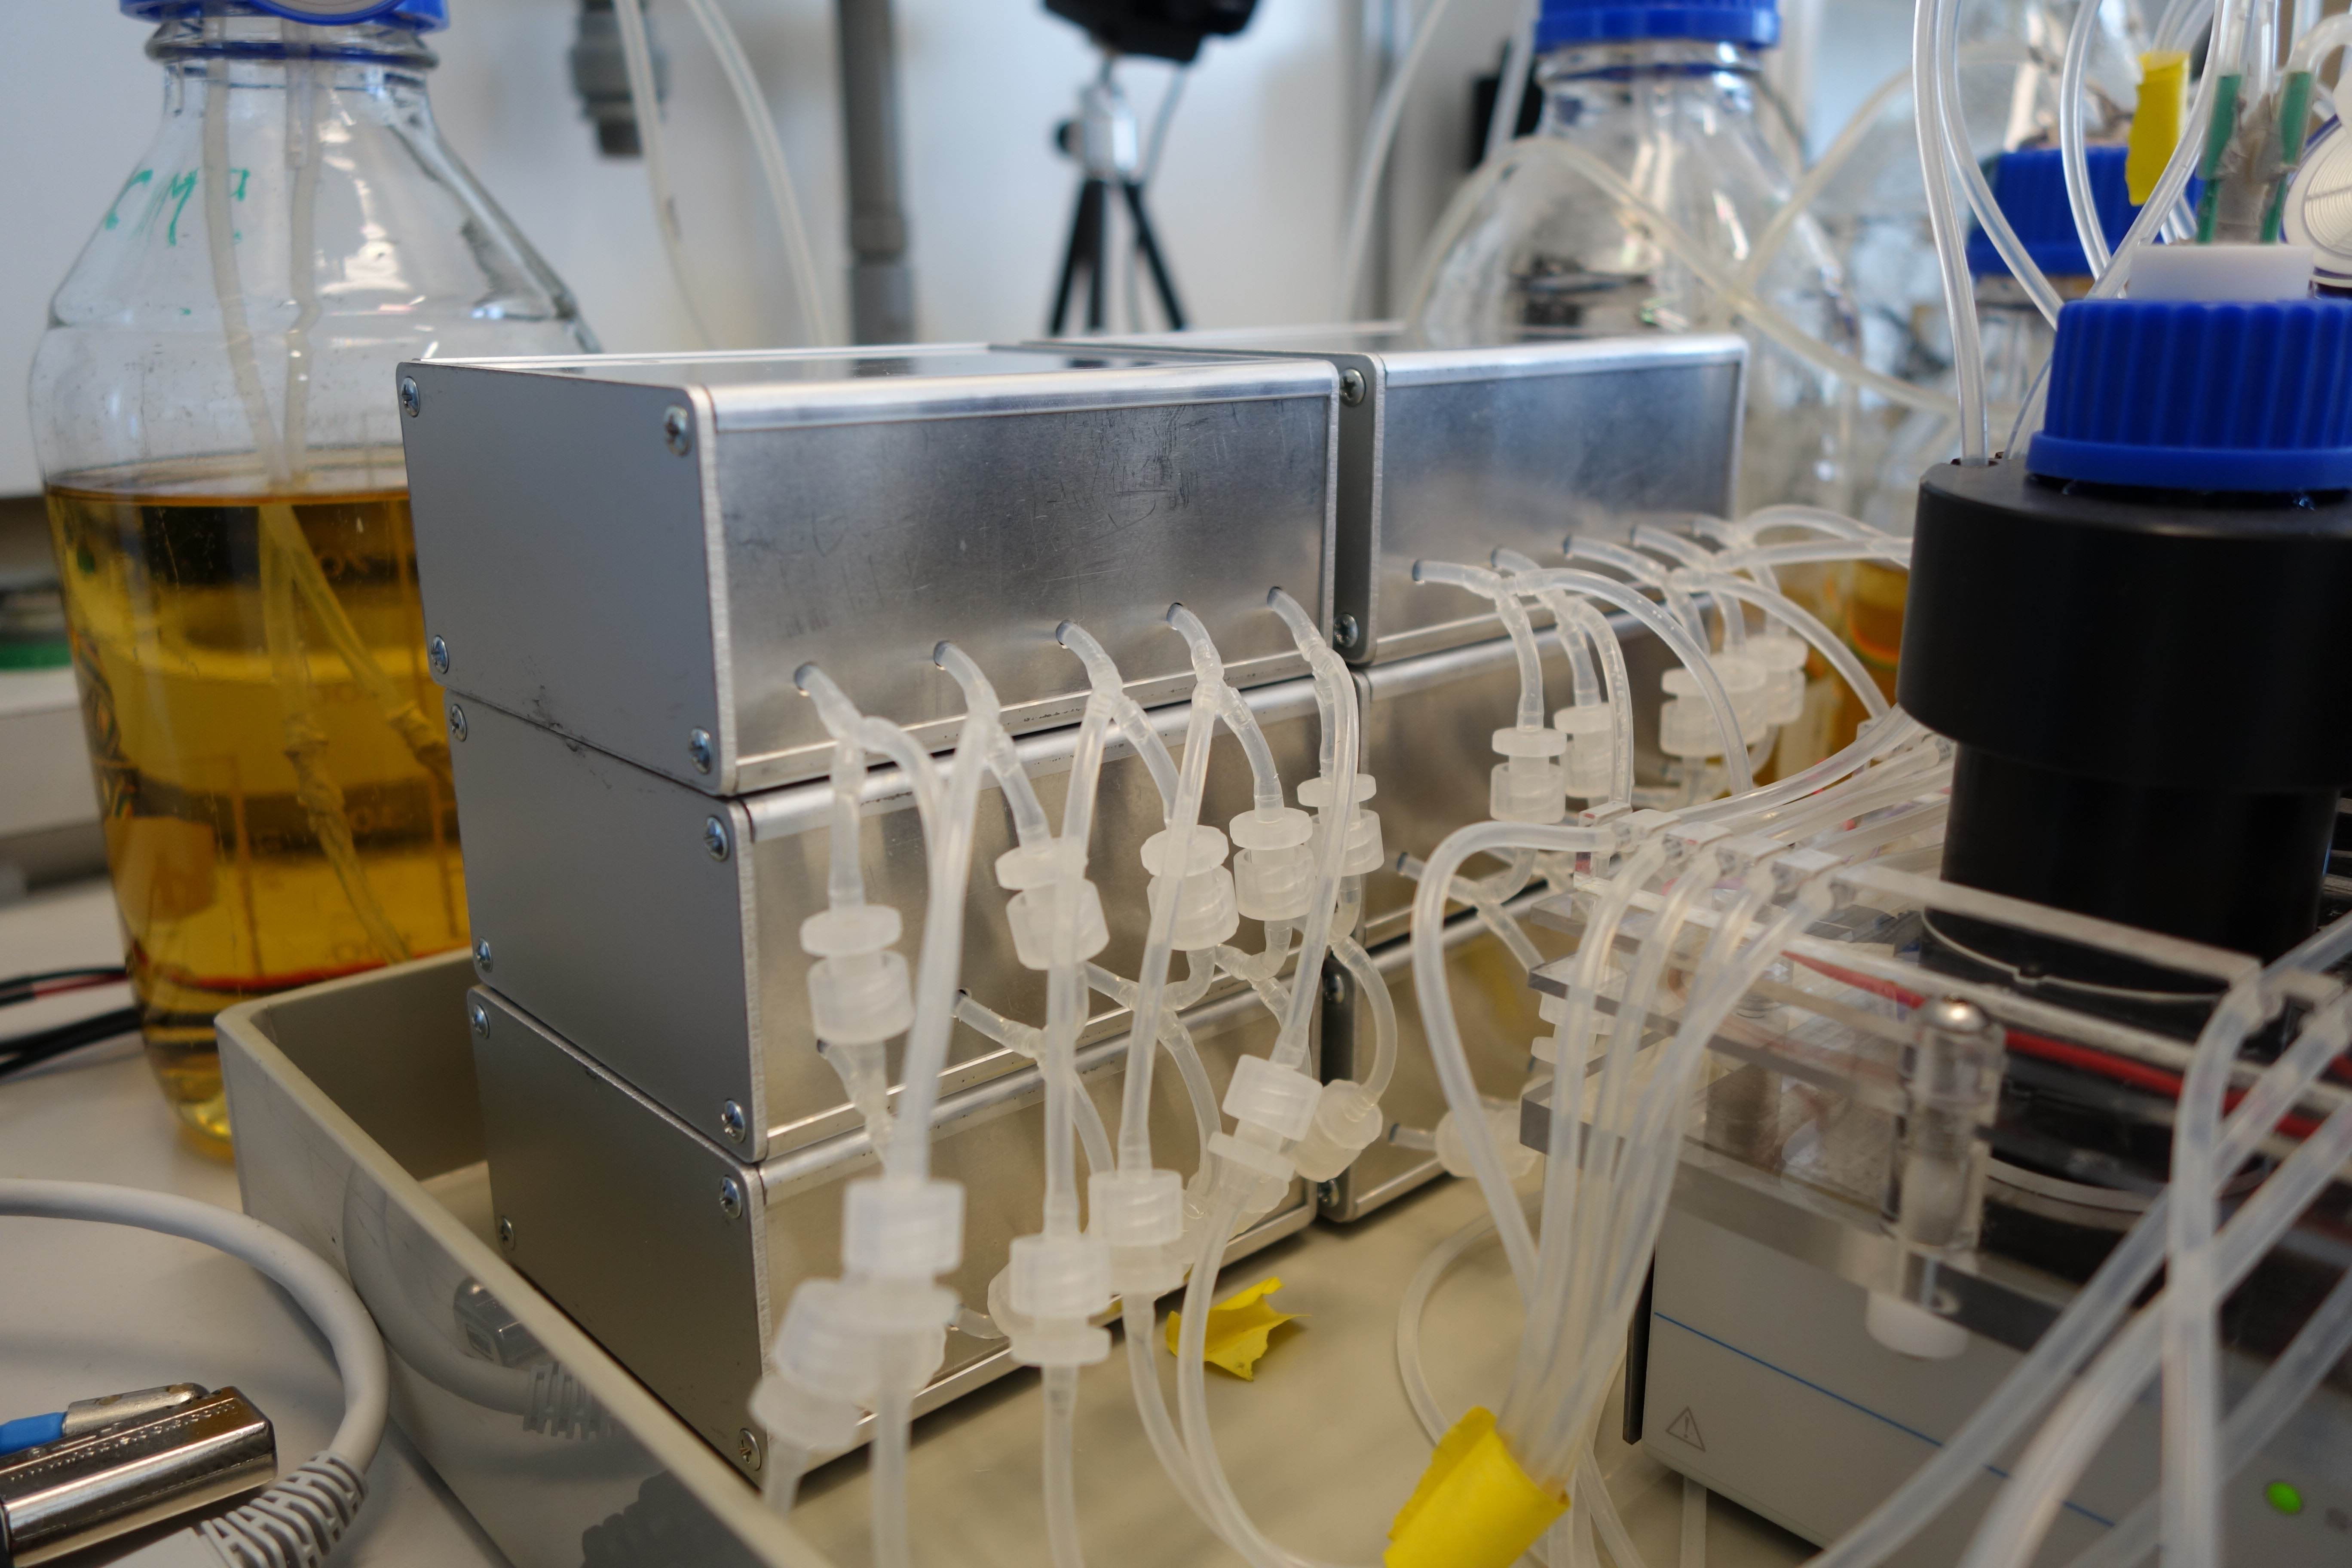
\includegraphics[scale=0.226]{pump_blocks.JPG}
	\caption{Figure left: Vial setup. Figure right: One row of five pumps represents one row of five vials. Since every vial is connected to three pumps, three rows of pumps are stacked on top of each other and connected column by column. This means that one column of three pumps is responsible for injection fluid into one vial. Every outlet from a pump from one column is connected, in order that there is just one tube going to one vial. }
	\label{figure:tubing_setup}
\end{figure}
Three connected injecting pumps per vial lead to 45 injecting pumps in total. Mp6 pumps from microComponents were chosen because they have a compact built, having the size of half an USB stick. 

The functional principle is based on a piezoelectric diaphragm in combination with passive check valves. By applying voltage the membrane is deformed, when the voltage decreases again the membrane drops down \cite{piezo_pumps}. Because the pump process depends on excitement and relaxation caused by the power, the flow rate generated by the pumps is dependent from the frequency. This also implements that the flow rate is very constant given that the power frequency is also constant. That being the case, the mixing of drug concentration was done by turning on the pumps for a calculated time.

In order to excite and relax the membrane and the piezopumps 230 Volts and a very steady power frequency were needed for this process, making it necessary to control every single pump with a specific mp6-OEM controller. This controller took an input power of 5 V and used about 30 mA of current. The Arduino was not capable of supplying this amount of current for every pump, therefor a separate power adapter was installed to supply the pumps. 

The pumps could be controlled by connecting one pin of the controller from the pump to a digital pin of the Arduino. 
If the pin from the controller was put to ground, the pumps were turned on, if the pin was connected to 5 V the pumps were off. Turning on/off the controller only worked well, when the change of power was very sudden. Unfortunately there was always a very small current flowing through the digital pins of the Arduino even when the pin was set to low. 
This caused problems with the controller of the pumps which could be solved by adding a pull-down resistor between the digital pins and the ground from the Arduino. Furthermore it was decided to work with a serial connected inverter, implementing that when the digital pin was set to low, the inverter caused a power of 5 V which meant that the pumps were off. On the other hand when the digital pin was set to high, the inverter produced a power of 0 V which turned the pumps on.  
As a waste pump a 16-channel peristalitc pump was used which was directly controlled with a digital pin from the Arduino. 
\begin{figure}
	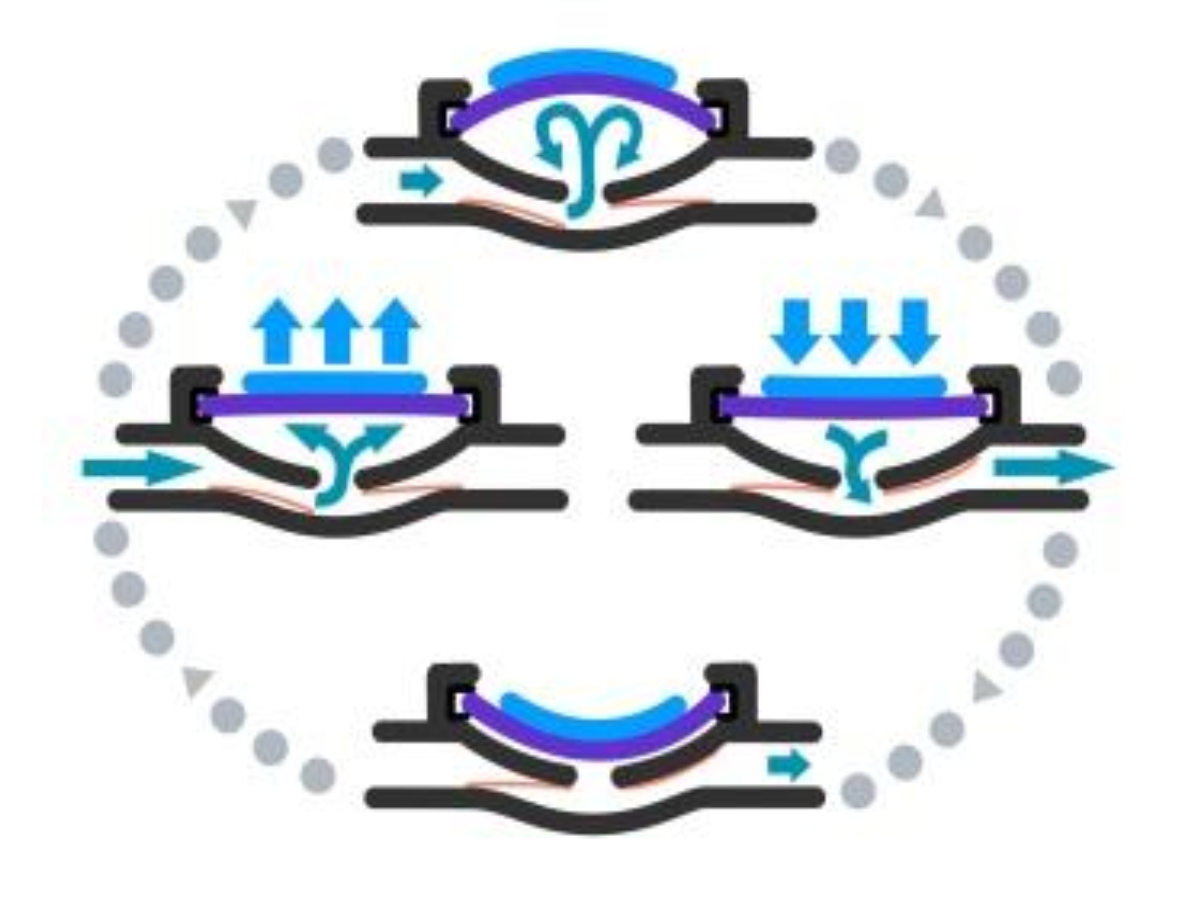
\includegraphics[scale=0.1]{piezo.png}
	%\includegraphics[]{circuit board}
	\caption{Principle of the mp6 pump but two of those piezoelectronics are connected in serial for this pump model \cite{piezo_pumps}}
	\label{figure:piezo}
\end{figure}

\subsection{control}
The controlling of the morbidostat was set up as an interaction of python programs running on a laptop and the .ino code running on the Arduino. The communication between the different types of code is possible because strings can be send with the arduino to the latop which can be interpreted with the serial package from python. On the other hand, strings sent from python can be intepreted with the Arduino. Even though it was necessary to thread the information sent with python in order to not create an overflow of commands on the arduino. 

There were mainly several python scripts running on the laptop, one called arduino\_interface.py which was handling the communication with the Arduino and another script called morbidostat\_experiment.py which was responsible for the feedback, meaning that it calculated the necessary runtimes of the pumps for each vial. This program was also responsible for constantly initiating the cycles. With a third script morbidostat\_setup.py the experiment was initialized at the beginning and with morbidostat\_monitor.py information produced from the morbidostat such as OD and drug injections could be monitored. Every script is available on \href{https://github.com/nahanoo/ESBL\_project/}{GitHub}. 
\begin{figure}[H]
	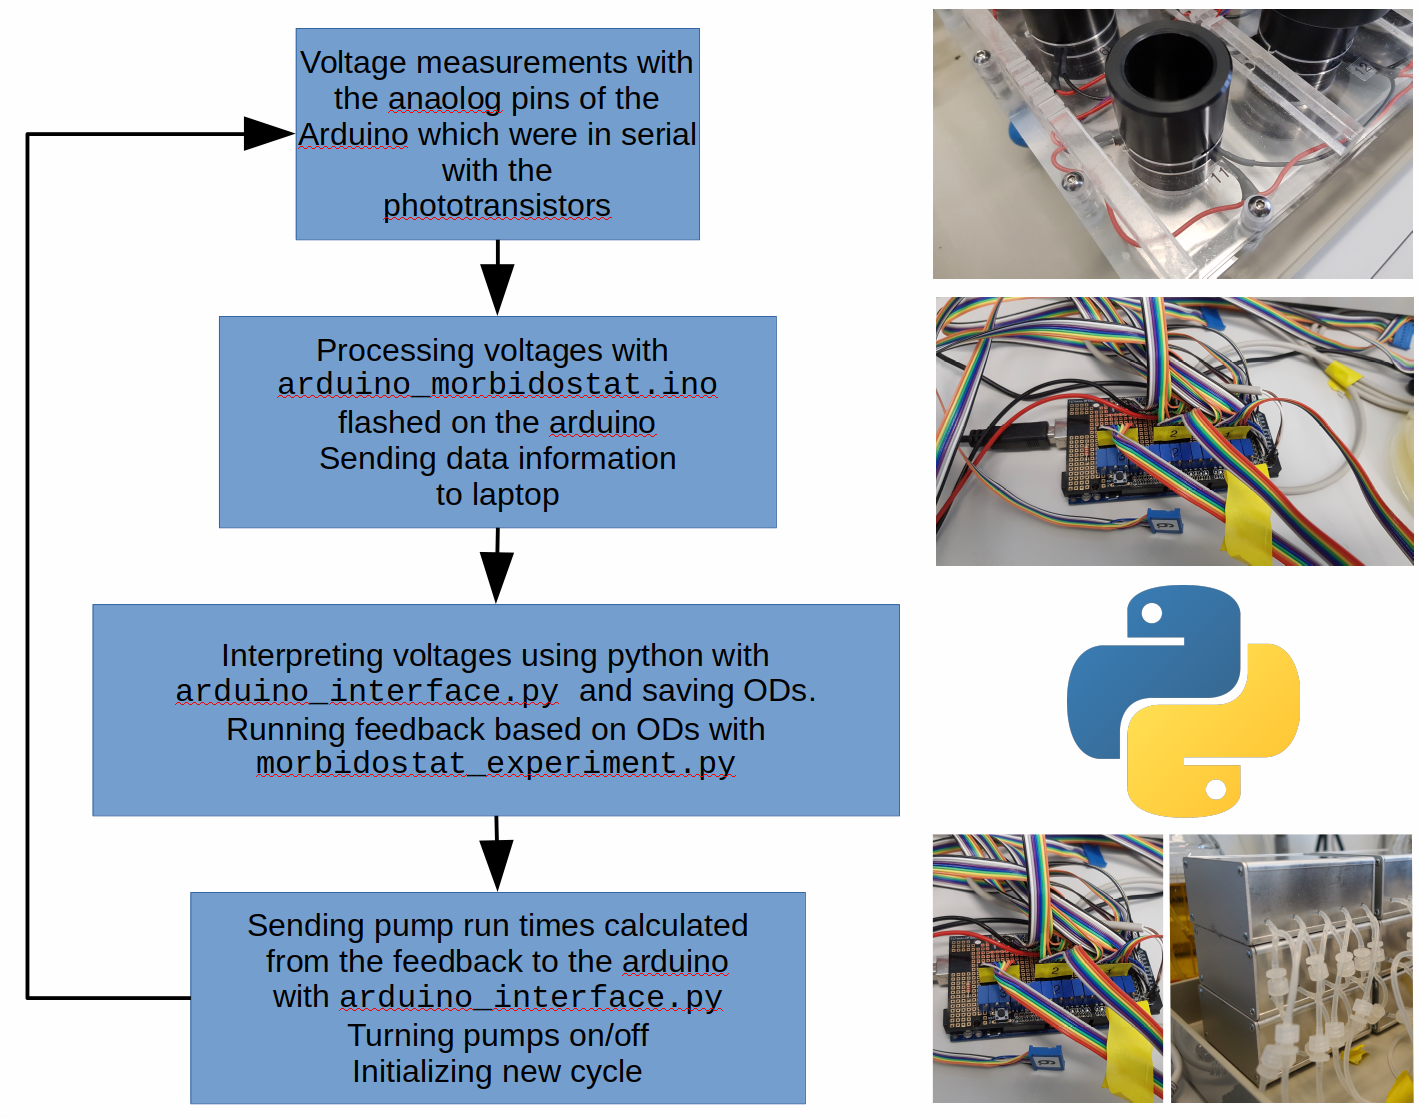
\includegraphics[scale=0.2]{flowchart.png}
	\caption{Overview of the morbidostat control. The arduino\_morbiostat.ino was running in a constant loop() measuring the currents for each vial. Threading had to be set up in the arduino\_interface.py in order that the Arduino didn't crash. The ODs and the injections could be monitored with morbidostat\_monitor.py. Changes in the control could be done by changing variables made possible by running morbidostat\_experiment.py in the interactive ipython mode.}
	\label{figure:flowchart}	
\end{figure}

\subsubsection{Feedback} 
For successfully putting the culture under antibiotic pressure it was a necessity to have a well working feedback which decided whether and how much drug was getting added to the culture. 
Every OD measurement in one cycle was averaged for every culture and called final OD. Using the final OD the growth of each culture could be described using following formula:
\begin{center}
	$\Delta OD = (final\_OD[x_{cycles \space back}] - final\_OD[Cycle_{current})/x$
\end{center}
It was important that the feedback didn't inject drug when the cultures were at a very low optical density because drug injection would may led to complete sterilization. Therefor a threshold was introduced which was called drug\_dilution\_therschold, which prevented drug injection if the final\_OD was below the OD defined in the drug\_dilution\_threshold.
Furthermore the goal of the feedback was to keep the cultures at defined OD. This desired OD was called target\_OD. Defining this OD was a trade off of having a higher probability of mutations for a higher defined target\_OD, but keeping the culture at a high OD implemented fewer accuracy of the OD measurement caused by many dead cells.  
Combining described variables above the feedback was implemented in morbidostat\_experiment.py as shown in \ref{figure:flowchart}:
\begin{figure}
	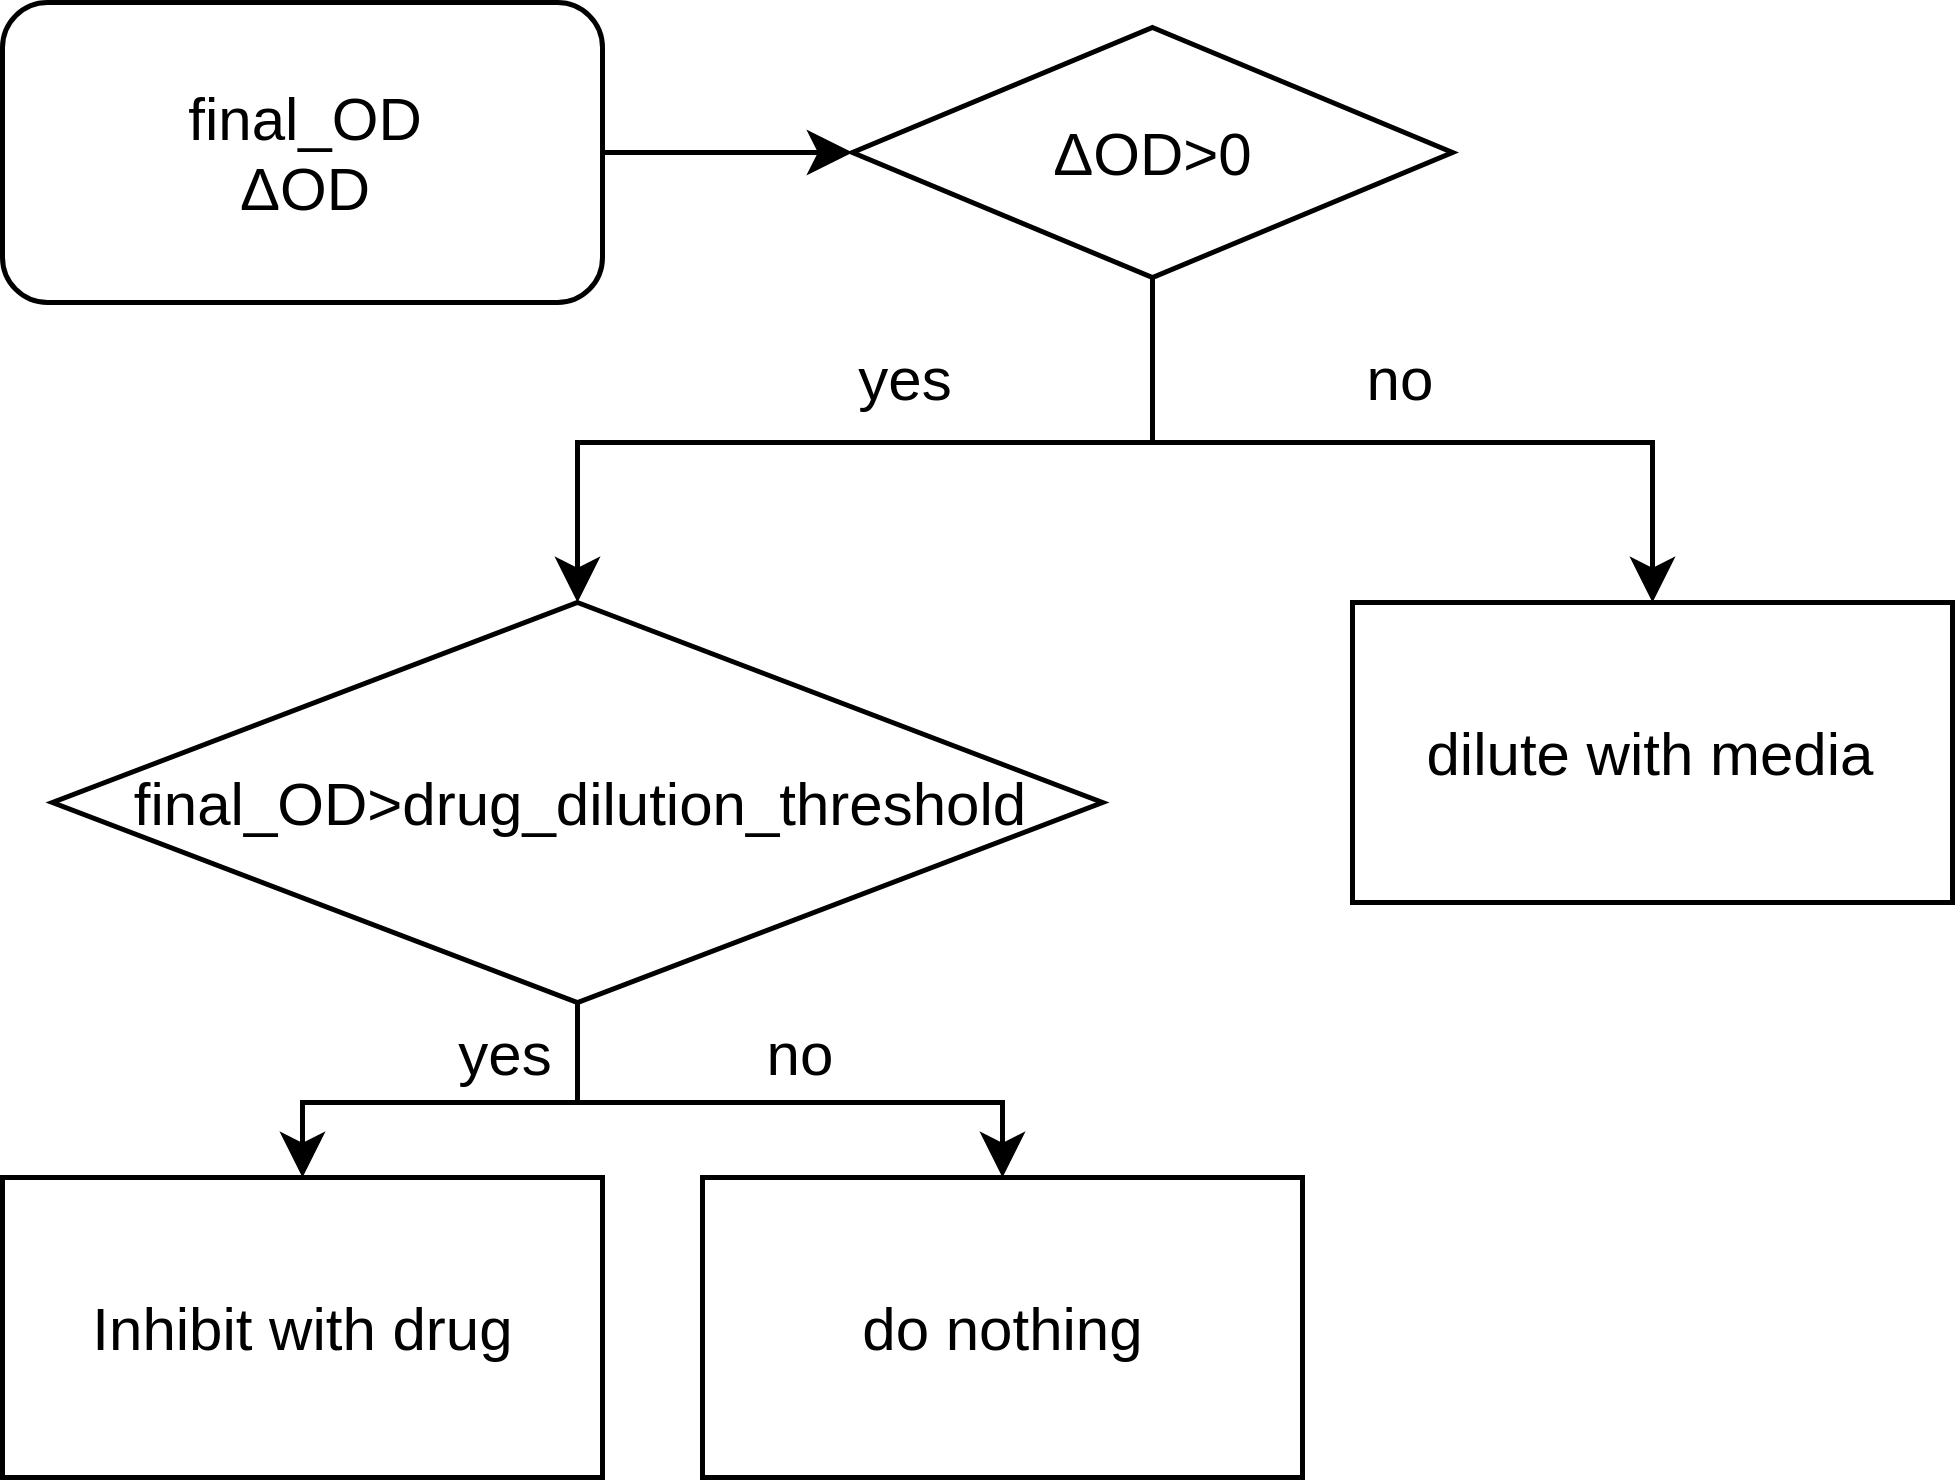
\includegraphics[scale=0.13]{feedback.png}
	\caption{If \textDelta OD is negative, implementing that the cells are dying, media is getting added in order to reduce drug concentration. If it's positive the final\_OD is compared to the drug\_dilution\_threshold, if it's bigger the cells are getting inhibited with drug, if it's smaller no liquid is added.}
	\label{figure:feedback}
\end{figure}

\subsection{Experimental procedure}
\subsubsection{OD and pump calibration}
As a media for all experiments a mixture of 1/10 LB media and 9/10 $H_2O$ was chosen. All the culturing of the bacteria was done in a 37 \degree \space incubator.  
For calibrating the OD measurements an overnight culure with K12 E. coli was inoculated in 5 ml diluted media. The next day the overnight culture was diluted 1/200 in 50 ml diluted media. After a few hours the OD of the culture was measured. Following ODs were prepared with 18 ml diluted media with the appropriate vials for the morbidostat: XXXXXXXXXXXXXXXXXXXXXXXXXXXXXX\\
Then every vial with of one certain OD was placed in every vial holder. With the function calibrate\_OD from the morbidostat\_experiment.py script, a current measurement was done for every OD and every vial holder. Because the current was measured for different ODs, the relation of current and OD could be described with a linear function. \\
For calibrating the pumps the function calibrate\_pumps from the morbidostat\_experiment.py was executed. This function demands the initial weight of every empty vial. After entering every weight, the function turned on every pump for 100 seconds. After that, the vials were weighted again and the values passed to the function which allowed precise calibration of each pump.

\subsubsection{MIC determination}
Since the feedback was heavily dependent on the MIC, this value had to be determined for every drug which was used to run the morbidostat. Therefor 5 ml of MHB media was inoculated with the bacteria used for the actual experiment and cultured over night. The next day a 1/200 dilution in 20 ml MHB was prepared and cultured for a few hours. In the mean while a 128 fold concentration of the MIC found in the literature for the drug of interest was prepared in MHB. 128 fold was chosen, because the determination was done in a 96 well plate which implements that the MIC found in the literature is in the middle of the plate. The growth of the diluted culture was constantly monitored by measuring the OD. When the OD of the diluted culture was at 0.08, a 1/100 dilution was done once again. From this final dilution 100 \textmu l was pipetted in every well from the 96 well expect in the wells from the last column of the plate. Additionally 100 \textmu l of MHB was added to every well. As a next step 100 \textmu l from the prepared drug solution was added to the first column of the plate. Then 100 \textmu l from this column was transferred to next column and mixed. This was repeated until the third last column. This implements that the second last column acts as a control of the cells, since no drug was added. The last column acts as a control for the media. After preparing the well plate it was incubated for 16 hours at 37 \degree \space and after that, the OD of every well was measured using a plate reader. As MIC the columnof a certain concentration which inhibited the culture significantly was chosen.
\label{section:mic_determination}


\subsubsection{Sterilization of the morbidostat}   
In order to prevent contamination a solution with sterile water containing 3 \% bleach was prepared and pumped through every pump for 5 minutes. After that we let the solution sit in the tubes for about an hour. Afer that every tube was flushed with sterile water by pumping it through every pump for 5 minutes. All the media, drug bottles and vials with its luer connections were autoclaved before the experiment.
\label{section:sterilization}

\subsubsection{Testing the continuous culture mode from the morbidostat}
An overnight culture was set up by inoculating 5 ml of diluted media with K12 XL1-Blue E. coli. The next day a 1/200 dilution in 200 ml was prepared and 18 ml of this suspension was pipetted in 18 sterile vials. A grow curve was determined by starting an experiment with the morbidostat in the GROWTH\_RATE\_EXPERIMENT modus. The morbidostat was put in the hypoxi-station at 37 \degree \space with an air composition of \_ \% $CO_2$ and \_ \% nitrogen. The growth rate experiment was done overnight. The next day ideal dilution rates for the continuous experiment were identified, by feeding the growth rates to the \href{https://github.com/nahanoo/ESBL\_project/}{morbidostat\_simulator.py} script which simulates a continuous morbidostat experiment. Also the best parameters for te feedback were determined using the simulator.
As a drug amoxicillin was chosen, it's MIC was determined as 2 \textmu/ml according to the procedure in \ref{section:mic_determination}. As a starting concentration 6 \textmu/ml and 14 \textmu/ml 
were chosen for the drug bottles. Tubing, bottles and vials were sterilized according to the section \ref{section:sterilization}. The continuous morbidostat experiment was started by initializing the experiment with the 	CONTINUOUS\_MORBIDOSTAT modus under the same temperature and air condition as for the grow curve determination. The dilution\_factor was set to 0.94. Every other day 200 \textmu of the suspension in the vials were transferred into new sterile vials filled with 18 ml diluted media. When a drug bottle was empty, the MIC was changed in the morbidostat\_experiment.py according to the concentration which was needed to strongly inhibit the growth. New drug concentrations were chosen based on the newly determined MIC. For the lower concentrated bottle a 3 fold MIC concentration, was chosen. For the higher concentrated drug bottle the concentration was set to 7 fold MIC. At day 4 of the experiment, samples were taken from every vial, by opening the vial in the hypoxi-station and transferring 200 \textmu into eppendorf tubes. Those samples were cultured over night in 5 ml diluted media and the next day the MIC was determined. The morbidostat experiment was stopped after 6 days.

\section{Plasmid construction}

 